% !TEX root = paper.tex
\section{Trip Identification}\label{s.trips}

Let the \emph{ith} sighting of vehicle \emph{k} be defined as the unordered pair:

\begin{equation} \label{e.sighting}
s^{k}_{i} = \{ c, t \}
\end{equation}

where \emph{c} is an integer that uniquely identifies a camera, and \emph{t} is a scalar representing a point in time (e.g.\ a timestamp).

Let an ordered sequence of sightings of vehicle \emph{k} define the \emph{uth} trip of \emph{k}:

\begin{equation} \label{e.trip}
w^{k}_{u} = \left(s^{k}_{(1)}, s^{k}_{(2)}, \dots , s^{k}_{(n)}\right)
\end{equation}

where \( n \) is the length of the trip, i.e.\ the number of sightings. Moreover, let the corresponding journey time sequence, of length \(n-1\), be defined as the time difference of consecutive sightings:

\begin{equation} \label{e.journeytime}
jt^{k}_{u} = \left(t^{k}_{(2)} - t^{k}_{(1)}, \ldots, t^{k}_{(n)} - t^{k}_{(n-1)} \right)
\end{equation}

We consider a trip of \emph{k} valid if the following conditions are met:

\begin{align}
n &\ge 1 , \label{e.trip.constraints.1} \\
\tau_{(i)} &< jt^{k}_{u(i)} < \Tau_{(i)} \ , \ \forall i \in jt^{k}_{u(i)} \label{e.trip.constraints.2}
\end{align}

The first condition~\ref{e.trip.constraints.1} is straightforward and specifies that every trip should have at least one sighting. The second condition~\ref{e.trip.constraints.2} defines a minimum and maximum travel times between consecutive observations. Its purpose is twofold:
\begin{enumerate*}[label=(\roman*)]
  \item first, to allow trips made by the same vehicle to be differentiated. For instance, given two consecutive sightings of \emph{k} three hours apart, we want to interpret them as belonging to different trips of \emph{k};
  \item second, it allows unplausible trips to be identified. For example, an unplausible trip can result from observing \emph{k} at a given camera and then a few seconds later at a second camera, several miles apart. Two explanations are common, either one of the cameras made a detection error, or there is another vehicle with a cloned plate number travelling in the road network.
\end{enumerate*} Evidently, condition~\ref{e.trip.constraints.2} is only valid for trips of length two or greater. Nevertheless, trips can easily be differentiated by first sorting sightings by time of occurrence, then calculating the journey time sequence for the entire sequence and finally comparing each element against $\Tau$. An example of a trip identified this way can be seen in Figure~\ref{fig:trip-example}.

\begin{figure*}[!ht]%
  \centering
  \begin{subfigure}[c]{.5\textwidth}
    \small
    \tabcolsep=0.09cm
    \begin{tabular}{c c c c c c c}
      \hline
      Vehicle & Camera & Timestamp & Trip & Sighting & \thead{Journey \\Time} & \thead{Trip \\Id}\\
      \hline
      2362920 & 1014 & \makecell{2017-02-01 \\ 00:00:06} &   1 &   1 & NA & 21 \\
      2362920 & 1044 & \makecell{2017-02-01 \\ 00:01:28} &   1 &   2 & 82.38 & 21 \\
      2362920 &  35 & \makecell{2017-02-01 \\ 00:02:32} &   1 &   3 & 63.50 & 21\\
      2362920 &  32 & \makecell{2017-02-01 \\ 00:04:38} &   1 &   4 & 125.95 & 21\\
       \hline
    \end{tabular}
    \label{fig:trip-example-table}
  \end{subfigure}\hfill
  %\qquad
  \begin{subfigure}[c]{.48\textwidth}
    \centering
    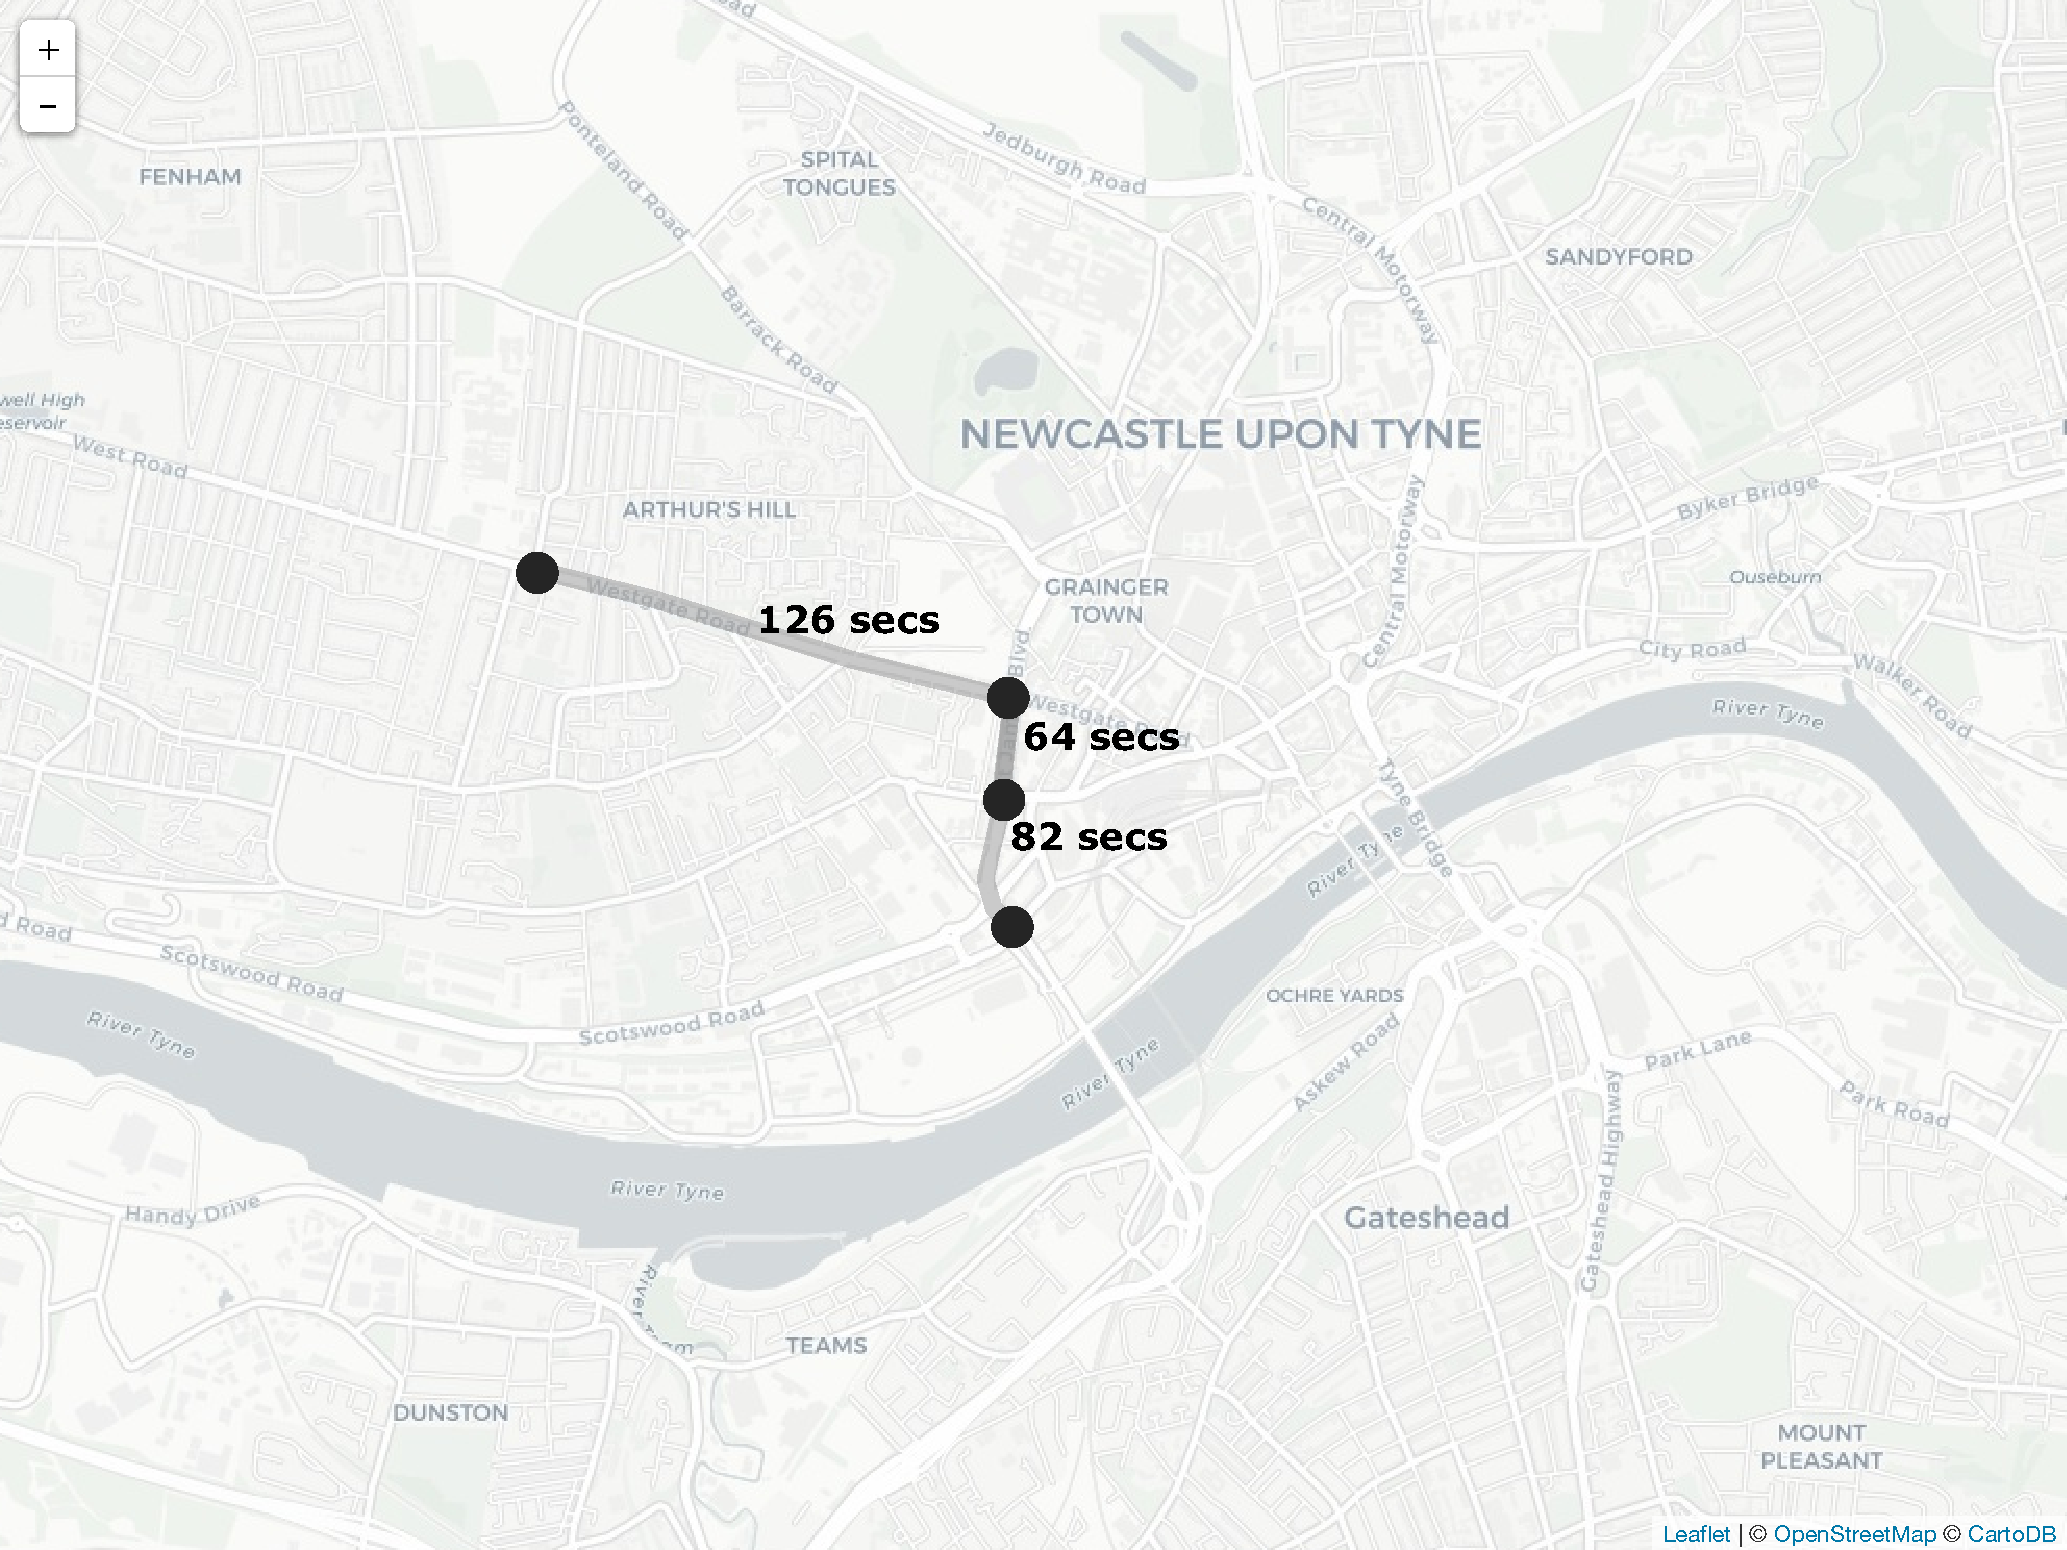
\includegraphics[width=1\linewidth]{trip-example.pdf}
    \label{fig:trip-example-map}
  \end{subfigure}\hfill
  \caption{Example of a trip of length 4. On the left side, w}%
  \label{fig:trip-example}%
\end{figure*}

The simplest approaching to choosing the value of $\Tau$ is to pick a fixed empirical value, such as 5 or 10 minutes. However, if the distance between two cameras is greater than another origin-destination (od) pair of cameras, then it makes sense that $\Tau$ is relaxed. Similarly, if there is an anomaly in the road network, such as a traffic jam, and the routes connecting the two cameras are affected, then the value of $\Tau$ should also be adapted. Hence, $\Tau_{(i)}$ should be a function of the distance between the two cameras (or, more accurately, of the top n-routes between these) and the distribution of observed journey times. The same rationale can be applied to estimating $\tau$. However, whilst devising methods to estimate $\Tau$ and $\tau$ under varying circumstances remains an open problem, it is something that we plan to work in the future. Thus, for the purposes of this work, we will consider these parameters to be fixed. Nevertheless, the importance of estimating these parameters should not be understated, as they are responsible for differentiating trips and identifying and filtering unplausible trips. Any errors that result from will propagate to the results and affect the outcome of the research. Figure~\ref{fig:length-dist} provides 

\begin{figure}[t]
  \centering
  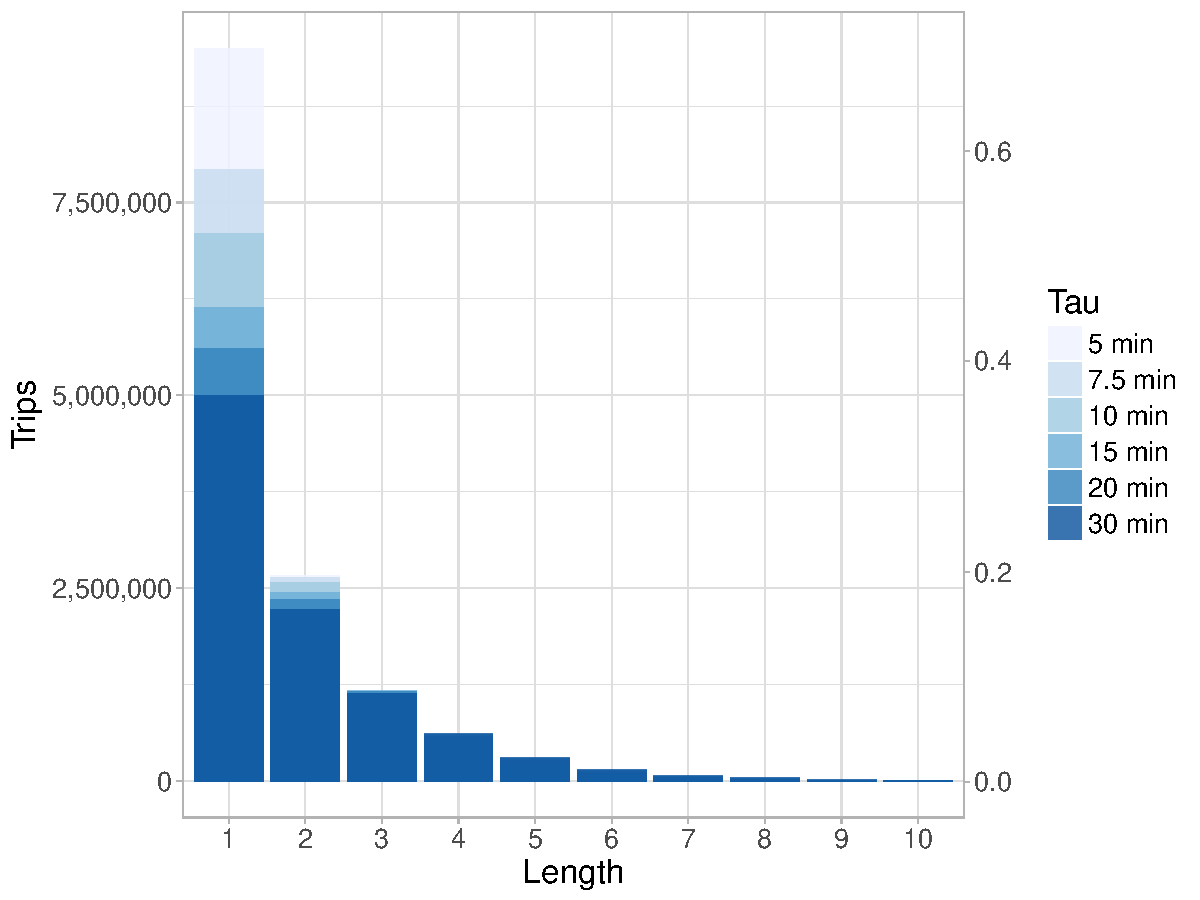
\includegraphics[width=1\linewidth]{length-dist.pdf}
  \caption{A}
  \label{fig:length-dist}
\end{figure}

\subsection{Duplicate scannings}

To ensure that every trip of vehicle \emph{k} is unique, the sequence of valid trips of vehicle \emph{k}:

\begin{align}
W^{k} = \left( w^{k}_{(1)}, w^{k}_{(2)}, \ldots, w^{k}_{(N)} \right) \label{e.trip.history}
\end{align}

where \emph{N} is the number of trips of \emph{k}, is such that there should be no two trips containing the same sighting:

\begin{align}
s^{k}_{(u(i))} \neq s^{k}_{(v(j))}, \forall u,v &= 1, 2, \ldots, N \ , \ u \neq v,  \label{e.trip.history.constraint} \\
\forall i,j &= 1, 2, \ldots, n \ , \ i \neq j \nonumber
\end{align}

where two sightings of vehicle \emph{k} are different simply if they were observed at two different points in time:

\begin{equation} \label{e.sighting.different}
t^{k}_{i} \ne t^{k}_{j} \Rightarrow s^{k}_{i} \ne s^{k}_{j} \ , \ i \ne j
\end{equation}

However, if these

then the two sightings are deemed as duplicates.

\subsection{Errors in plate scanning}
